\section{Durchführung}
\label{sec:Durchführung}
Es werden drei Messungen mit unterschiedlichen Messaufbauten aufgenommen, um die Bedienung des Lasers zu üben.
Aus Sicherheitsgründen wurden Schutzbrillen getragen und, um die Messungen so störfrei wie möglich zu machen,
wurde der Raum teilweise abgedunkelt.

\subsection{Messen des Schwellenstrom}
\label{sec:Schwellenstrom}
Für den weiteren Versuch ist es wichtig den Schwellenstrom zu messen, da unter dem Schwellenstrom der Laser nur
als LED funktioniert und dementsprechend kein kohärents Licht erzeugt. Dafür wird der Laser an eine Apparatur
angeschlossen mit der der Strom variiert werden kann. Weiterhin wird eine Kamera vor eine Detektorkarte
positioniert, der Strom notiert bei dem Lasergranulation auftritt und entsprechende Fotos gemacht. Der
entsprechend Aufbau ist in \autoref{fig:aufbau1} zu finden.
Die Detektorkarte wird so positioniert, dass der Strahl auf sie auftrifft. Lasergranulation (auch Speckle genannt)
ist ein Beugungseffekt, der durch die Unebenheit der Detektorkarte entsteht und ist leicht durch ein gepunktetes
Muster um die Auftreffstelle des Laserstrahls zu erkennen.

\begin{figure}
    \centering
    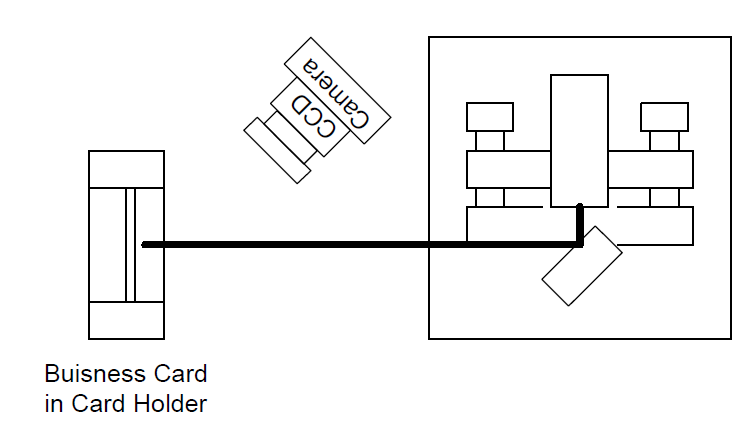
\includegraphics[height=6cm]{content/pics/aufbau1.png}
    \caption{Schematische Darstellung des Aufbaus zur Messung des Schwellenstroms. \cite{V60}}
    \label{fig:aufbau1}
\end{figure}

\subsection{Aufnahme der Rubidiumsfluoreszenz}
\label{sec:Rubidium}
Um Rubidiumfluoresenz zu erreichen, wird ein in \autoref{fig:aufbau2} abgebildeter Aufbau verwendet. Dabei wird
Laserlicht auf eine Rubidiumzelle gerichtet, so dass das Rubidium angeregt wird und auf der Kamera erkennbar ist.
Für die restlichen Messungen wird ein Strom über dem Schwellenstrom eingestellt.
Da eine bestimmte Frequenz benötigt wird, um das Rubidium anzuregen, wird die Frequenz mit Hilfe eines
winkelverstellbaren Gitters variiert. Weiterhin kann zum Erreichen der Frequenz auch der Strom des Piezokristalls
am Controller verändert werden.

\begin{figure}
    \centering
    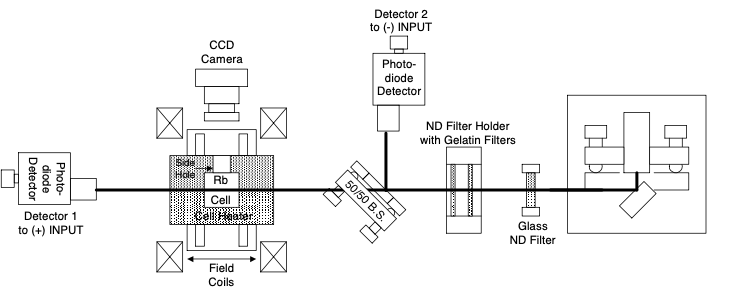
\includegraphics[height=6cm]{content/pics/aufbau.png}
    \caption{Schematische Darstellung des Aufbaus zur Messung der Rubidiumsfluoreszenz. \cite{V60}}
    \label{fig:aufbau2}
\end{figure}

\subsection{Transmissionsspektrum der Rubidiumzelle}
\label{sec:Transmissionsspektrum}
Um das Transmissionsspektrum von Rubidium zu bestimmen, wird wieder der Aufbau in \autoref{fig:aufbau2} verwendet.
Diesmal wird zusätzlich das Signal der Photodetektoren benötigt. Hinter der Rubidiumzelle wird ein 
50/50-Strahlteiler montiert, der den Strahl auf eine Photodiode lenkt. Eine weitere Photodiode, an der das
tatsächliche Spektrum gemessen wird, wird hinter dem Strahlteiler installiert. Durch einen Funktionsgenerator können
beide Signale der Photodioden verrechnet werden, um ein möglichst gleichmäßiges und geringes Hintergrundrauschen
zu haben. Das wird durch ein angeschlossenes Oszilloskop abgelesen.